 \begin{marginfigure}[-20mm]
  \centering
    \caption[-0mm]{Figure~3 from the paper\tss{\ref{ref:1} } \label{fig:paperfig3}} 

  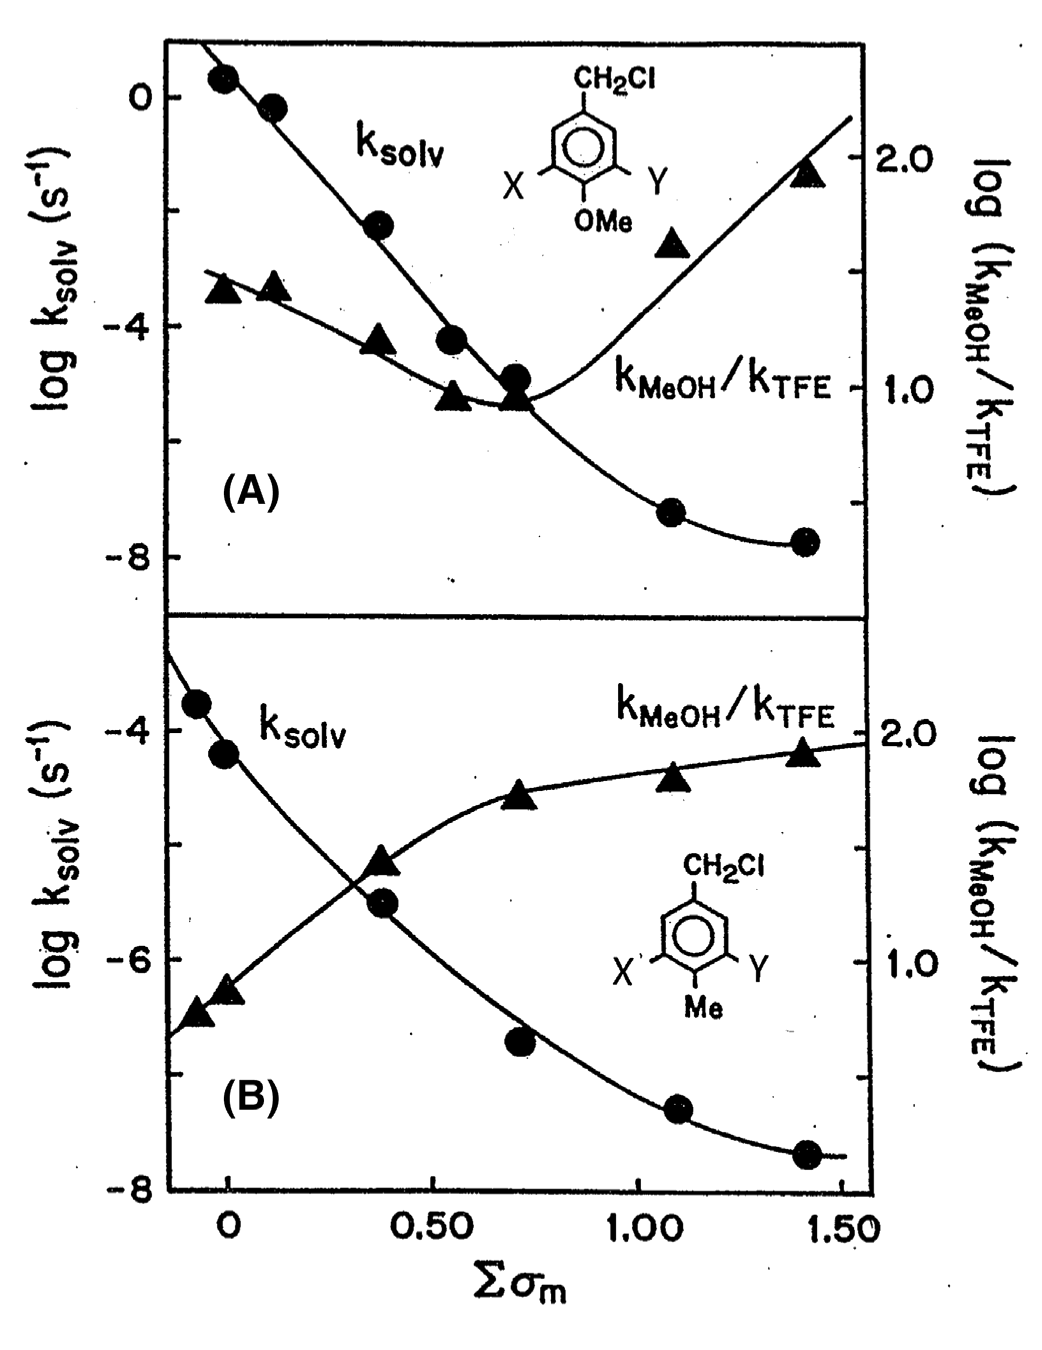
\includegraphics[width=150pt]{images/fig3paper.png}
  
  
\end{marginfigure}

 \begin{marginfigure}[0mm]
  \centering
    \caption[-0mm]{Figure~4 from the paper\tss{\ref{ref:1}} \label{fig:paperfig4}}  

  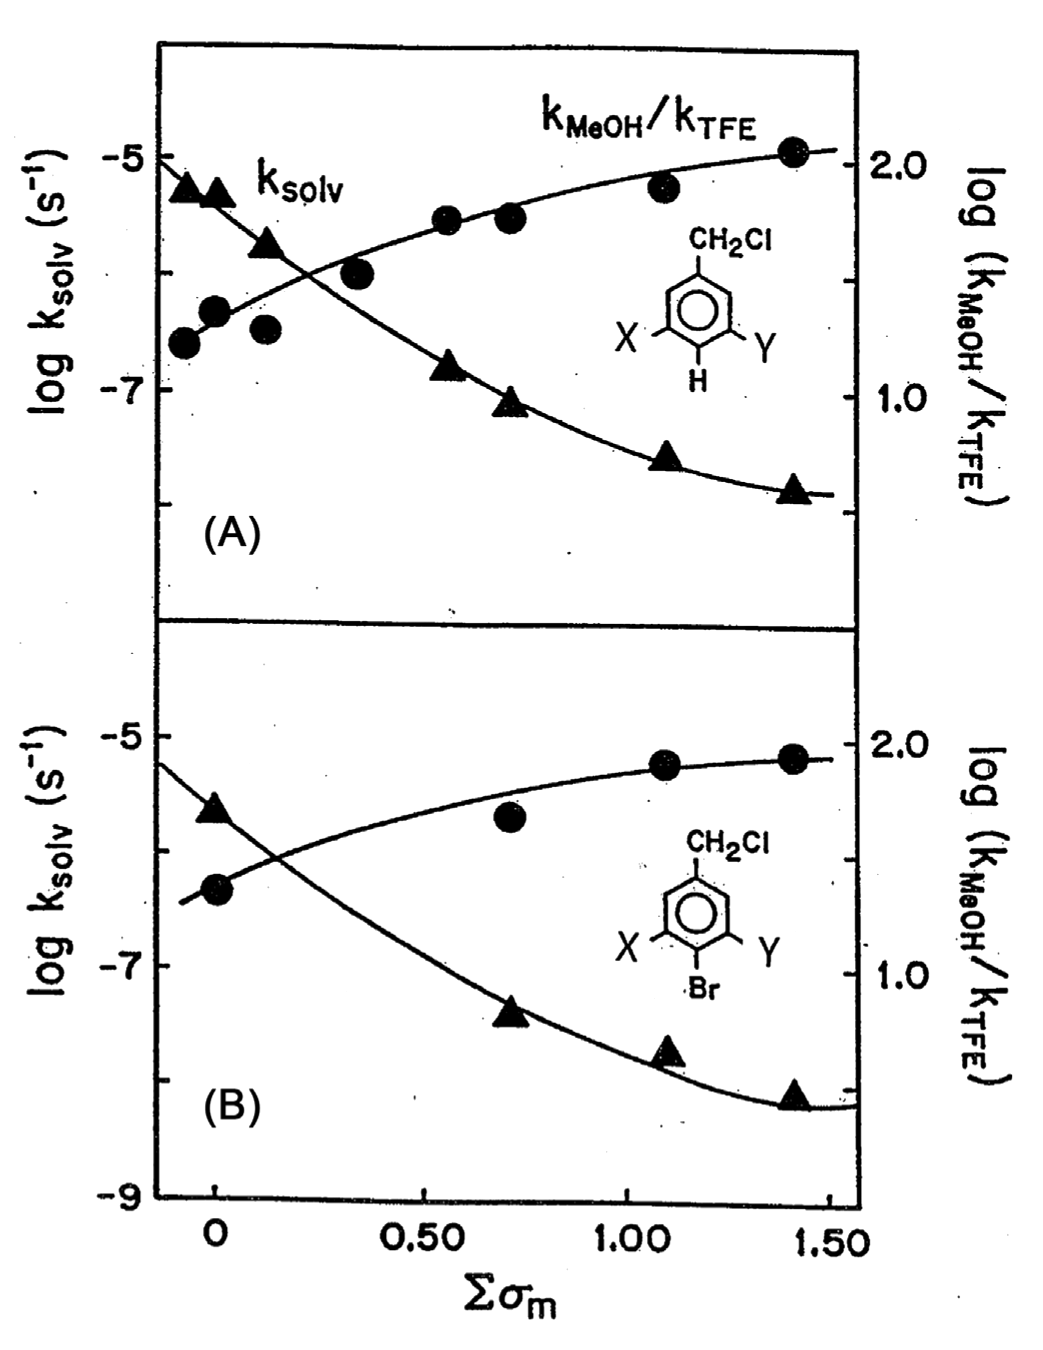
\includegraphics[width=150pt]{images/fig4paper.png}
  
  
\end{marginfigure}



The authors present the data from tables~\ref{tab:1} and \vref{tab:2} in a pair of plots where the $\log{k_{obs}}$ is plotted agains the sum of substituent effects for \textit{meta} substituents in each separate set of \textit{para}-substituted benzyl chlorides, \ce{p-OMe}, \ce{p-Me}, \ce{p-H}, and \ce{p-Br}. They do not present results for \ce{p-NO2} in these plots as there are only two data points for that case.

We expect a negative reaction constant, $\rho$, of high magnitude for the $S_N1$ mechanism where the rds is formation of the carbocation intermediate. The $S_N2$ mechanism is expected have a negative value with a much smaller magnitude for $\rho$. The authors use the extended Hammett equation and will present two separate values for $\rho$, the reaction constants for inductive effects, $\rho_n$, and for resonance effects, $\rho_r$.

\subsection{The Authors Plots}
In the figures from the paper (reproduced in figures~\ref{fig:paperfig3} and \vref{fig:paperfig4}) we see that the \ce{p-OMe} series has a steep negative slope against $\sum \sigma_m$. The slopes in the other three cases are less negative. The authors also present the solvent nucleophile selectivity data on the same plots. I will discuss these results later. Do pause to note that the circles represent $\log{k_{obs}}$ data is the first plot and $\nicefrac{k_{MeOH}}{k_{MeOH}}$ in the second. If you check the figure legends in the paper\tss{\ref{ref:1} } you will see that the authors intended to use the circles for $\log{k_{obs}}$ in both plots. This discrepancy should have been caught by the editors. 

It is difficult to compare the four sets of results visually because they are presented in four separate plots with different scales so I will plot all data in a single plot in my own analysis. The curves on the plots have no meaning and are meant to help the reader visually interpret the plots. 

\subsection{My Own Plots}
I will now use the data and the methods of the authors and will hopefully obtain nearly identical values for $\rho_n$ and $\rho_r$ using the extended Hammett equation. I will plot the values for $\log{k_{obs}}$ against $\sum \sigma_m$ for all five sets on the same plot.\sidenote[][0mm]{The code for generating the plots is available as a \textit{Python} notebook that accompanies this document. You will be able to see exactly how I calculated values for $\sum \sigma_m$ and how I created the line fits on the plots.}








\begin{algorithmic}
\State $i \gets 10$
\If{$i\geq 5$} 
    \State $i \gets i-1$
\Else
    \If{$i\leq 3$}
        \State $i \gets i+2$
    \EndIf
\EndIf 
\end{algorithmic}
